\documentclass[12pt,a4paper]{article}
\def\qe{{\sc Quantum ESPRESSO}}
\usepackage{amssymb}
\usepackage{graphicx}
\usepackage{hyperref}
\usepackage{amsmath}
\pagestyle{plain}
\textwidth = 15.5 cm
\textheight = 23.5 cm
\topmargin =-1.0 cm
\oddsidemargin = 0.5 cm
\listparindent=0pt
\itemsep=5pt

\begin{document} 
\title{Quick reference guide on \texttt{PLUMED} with \qe}
\author{{\em Changru Ma}\\
SISSA, Trieste\\
}
\date{March 30, 2011}
\maketitle
\tableofcontents
\newpage

\section{Introduction}

\texttt{PLUMED}\cite{Bonomi:2009ul} is a plugin for free energy calculation in molecular systems which works together with some of the most popular molecular dynamics engines, including classical (GROMACS, NAMD, DL\_POLY, AMBER and LAMMPS), GPU-accelerated (ACEMD) and ab-initio (\qe) codes.

Free energy calculations can be performed as a function of many order parameters with a particular focus on biological problems using state of the art methods such as metadynamics\cite{Laio:2008wu}, umbrella sampling and Jarzynski-equation based steered MD.

The software, written in ANSI-C language, can be easily interfaced with both fortran and C/C++ codes.

The \texttt{PLUMED} user guide can be downloaded here

\href{https://sites.google.com/site/plumedweb/documentation}{https://sites.google.com/site/plumedweb/documentation}

and \texttt{PLUMED} tutorial can be found here

\href{http://sites.google.com/site/plumedtutorial2010/}{http://sites.google.com/site/plumedtutorial2010/}. \\

{\bf All the features in \texttt{PLUMED} are compatible with \qe\ but:}

\begin{itemize}
\item variable cell calculations
\item non-orthorhombic cell
\item energy related collective variables
\end{itemize}

\subsection{Overview}

A system described by a set of coordinates $x$ and a potential $V(x)$ evolving under the action of a dynamics whose equilibrium distribution is canonical at a temperature $T$. We explore the properties of the system as a function of a finite number of CVs $S_{\alpha}(x), ~\alpha ~= ~1, ~d$. The equilibrium behavior of these variables is defined by the probability distribution

\begin{equation}
P(s)~=~\frac{exp(-(1/T)F(s))}{\int{ds~exp(-(1/T)F(s))}}
\label{EQ_prob}
\end{equation}

where $s$ denotes the d dimensional vector $(s_{1},..., ~s_{d})$ and the free energy is given by

\begin{equation}
F(s) ~= ~T ~ln(\int{dx ~exp(-\frac{1}{T}V(x))} ~\delta(s-S(x)))
\label{EQ_free_energy}
\end{equation}

Here capital $S$ is used for denoting the function of the coordinates $S(x)$, while lower case s is used for denoting the value of the CVs.

In metadynamics the free energy is reconstructed recursively, starting from the bottom of the well by a history-dependent random walk that explores a larger and larger portion of configuration space. A small repulsive Gaussian potential is added every $\tau_{G}$ MD steps. The external ('metadynamics') potential acting on the system at time $t$ is given by

\begin{equation}
V_{G}(S(x), ~t) ~= ~\omega ~\sum_{\substack{t' ~= ~\tau_{G}, ~2\tau_{G},...\\t'<t}}exp(-\frac{(S(x)-s(t'))^{2}}{2\delta s^{2}})
\label{EQ_vg}
\end{equation}

where $s(t) = S(x(t))$ is the value of CV at time $t$. Three parameters enter the definition of the $V_{G}$ are the Gaussian height $\omega$, the Gaussian width $\delta s$ and the frequency $\tau_{G}$ at which the Gaussians are added.

If the Gaussians are large, the free energy surface will be explored at a fast pace, but the reconstructed profile will be affected by large errors. Instead, if the Gaussians are small or are placed infrequently the reconstruction will be accurate, but it will take a longer time.

A hint of the two different manners in which metadynamics can be used:

\begin{itemize}
\item It can be used to 'escape free energy minima, i.e. to find the lowest free energy saddle point out of a local minimum. In this case the metadynamics should be stopped as soon as the walker exits from the minimum and starts exploring a new region of space.
\item It can be used to exhaustively explore a predefined region in the CV space and reconstruct the free energy surface. In this case the simulation should be stopped when the motion of the walker becomes diffusive in this region.
\end{itemize}

The basic assumption of metadynamics is that $V_{G}(s, t)$ after a sufficiently long time provides an estimate of the underlying free energy $\lim_{t \to \infty} V_{G}(s, t) ~  -F(s)$. This equation states that an equilibrium quantity, namely the free energy, can be estimated by a non-equilibrium dynamics in which the underlying potential is changed every time a new Gaussian is added.

If the CV is a $d$-dimensional vector, namely two or more CVs are used at the same time, the metadynamics potential is given by

\begin{equation}
V_{G}(S(x), t) ~=~ \omega \sum_{\substack{t' ~= ~\tau_{G}, ~2\tau_{G},...\\t'<t}}exp(- \sum_{\alpha = 1}^{d} \frac{(S(x)-s(t'))^{2}}{2\delta s^{2}})
\label{EQ_vgd}
\end{equation}

and it is necessary to choose a width $\delta s_{\alpha}$ for each CV. Metadynamics works properly only if $d$ is small, and that the quality of the reconstructed free energy is strongly influenced by the parameters $\omega$ and $\delta s$. Large values for $\omega$ and $\delta s$ allow for a fast sampling of the CV space at the price of a low accuracy.

For a detailed description, please see the references Laio {\it et al.}\cite{Laio:2008wu, Laio:2002wm}.

\subsection{Collective variables}
The reliability of metadynamics is strongly influenced by the choice of the CVs. Ideally the CVs should satisfy three properties:

\begin{itemize}
\item They should clearly distinguish between the initial state, the final state and the intermediates.
\item They should describe all the slow events that are relevant to the process of interest.
\item Their number should not be too large, otherwise it will take a very long time to fill the free energy surface.
\end{itemize}

If the free energy grows 'smoothly' it is likely that the set of variables is complete. \\

{\bf CVs compatible with \qe~ are, for instance:}

\begin{itemize}
\item Geometry-related variables. Such as distances, angles and dihedrals formed by atoms or groups of atoms. These variables are frequently used in the study of chemical reactions and biophysical systems.
\item Coordination numbers. It can be used to detect the presence of a bond between two atoms or for counting the bonds between two different atomic species.
\end{itemize}

For a complete list of CVs implemented in \texttt{PLUMED}, please have a look at the \texttt{PLUMED} reference manual.
{\bf Energy related CVs are not compatible with \qe}.


\section{Step-by-step metadynamics calculations}

\subsection{Compile \qe\ with \texttt{PLUMED} plugin}

In this section, we will show how to compile \qe\ with \texttt{PLUMED} plugin.
First of all, one of the following versions of the source package has to be 
downloaded:

\begin{itemize}
\item \qe\ release 4.3
(\href{http://qe-forge.org/gf/project/q-e}{http://qe-forge.org/gf/project/q-e}),
 follow link "Files" on the left)
\item SVN version (link as above, follow link "SVN" on the left)
\end{itemize}

To install \qe\ from source, you need first of all a minimal Unix environment: basically, a command shell (e.g., bash or tcsh) and the utilities make, awk, sed. Second, you need C and Fortran-95 compilers. For parallel execution, you will also need MPI libraries and a ``parallel'' (i.e. MPI-aware) compiler. For massively parallel machines, or for simple multicore parallelization, an OpenMP-aware compiler and libraries are also required.\cite{QE:guide}.

Then you need to run the \texttt{configure} script as usual. After the successful configuration, just type \texttt{make plumed}. \texttt{make plumed} just untar \texttt{PLUMED-latest.tar.gz}, move to \texttt{PLUMED} directory just under \texttt{espresso}, patch \texttt{PW} and \texttt{CPV} files and recompile \texttt{PW}, \texttt{CPV} and \texttt{clib}. Please note that, do not try \texttt{make all}, that will compile the code without the \texttt{PLUMED} plugin.

Instructions for the impatient:

\begin{verbatim}
cd espresso-X.Y.Z/
./configure
make plumed
\end{verbatim}

\subsection{Running metadynamics in \qe}

To run the metadynamics calculations, you will need to prepare the input file \texttt{plumed.dat} for \texttt{PLUMED} (see \texttt{PLUMED} manual\cite{PLUMED:manual} for a detailed description), that should be located in \texttt{outdir} and the standard input file for \qe. And then, you may execute the program as usual but with a flag \texttt{-plumed}.

For Born-Oppenheimer Molecular Dynamics,

\begin{verbatim}
pw.x -plumed < pw.in > pw.out
\end{verbatim}

for Car-Parrinello Molecular Dynamics,

\begin{verbatim}
cp.x -plumed < cp.in > cp.out
\end{verbatim}

\subsection{Units in the input and output files}

There are several output files for the simulation with \texttt{PLUMED}, e.g. \texttt{PLUMED.OUT}, \texttt{COLVAR} and \texttt{HILLS}. All the units in the input and output files for \texttt{PLUMED} adopt the internal units of the main code, say Rydberg atomic units in \texttt{pw.x} and Hartree atomic units in \texttt{cp.x}. But there are two exceptions, for distance it is always Bohr and for energy it is always Rydberg.

\subsection{Postprocessing}

There is a \texttt{sum\_hills.f90} code (in espresso/PLUMED/utilities/sum\_hills/) performing post-processing task to estimate the free energy after a metadynamics run. The program \texttt{sum\_hills.f90} is a tool for summing up the Gaussians laid during the metadynamics trajectory and obtaining the free energy surface.

As \texttt{sum\_hills.f90} is a simple fortran 90 program, the installation is straight- forward so long as you have a fortran compiler available on your machine. As an example, with the gnu g95 compiler one would compile sum hills.f90 using the following command:

\begin{verbatim}
g95 -O3 sum_hills.f90 serial.f90 -o sum_hills.x
\end{verbatim}

For post processing of large HILLS files it is recommended to use a parallel version.

The \texttt{sum\_hills.x} program takes its input parameters from the command line. If run without options, this brief summary of options is printed out. Detail descriptions of the following options can be found in the manual\cite{PLUMED:manual} of \texttt{PLUMED}.

\begin{verbatim}
USAGE:
sum_hills.x -file HILLS -out fes.dat -ndim 3 -ndw 1 2 -kt 0.6 -ngrid 100 100 100
[-ndim 3         ] (number of collective variables NCV)
[-ndw 1 ...      ] (CVs for the free energy surface)
[-ngrid 50 ...   ] (mesh dimension. DEFAULT :: 100)
[-dp ...         ] (size of the mesh of the output free energy)
[-fix 1.1 ...    ] (define the region for the FES, if omitted this is 
                   automatically calculated)
[-stride 10      ] (how often the FES is written)
[-cutoff_e 1.e-6 ] (the hills are cutoff at 1.e-6)
[-cutoff_s 6.25  ] (the hills are cutoff at 6.25 standard deviations from
                   the center)
[-2pi x          ] ([0;2pi] periodicity on the x CV, if -fix is not used 2pi
                   is assumed)
[-pi x           ] ([-pi;pi] periodicity on the x CV, if -fix is not used 2pi
                   is assumed)
[-kt 0.6         ] (kT in the energy units)
[-grad           ] (apply periodicity using degrees)
[-bias <biasfact>] (writing output the bias for a well tempered metadynamics run)
[-file HILLLS    ] (input file)
[-out  fes.dat   ] (output file)
[-hills nhills   ] (number of gaussians that are read)
\end{verbatim}

\section{First worked example: SN2 reaction}

\subsection{SN2 reaction in vacuum}

In this section, we will show a very simple chemical reaction done with \qe\ code with \texttt{PLUMED} plugin. The goal of this example is to study the free energy for the reaction depicted in Fig. \ref{Fig_Reaction_sn2}. This SN2 reaction between Cl$^{-}$ and CH3Cl shows the symmetric transition state and the CH3 conversion of configuration known as the Walden inversion\cite{Ensing:2005p53}.

\begin{figure*}[htbp]
\begin{center}
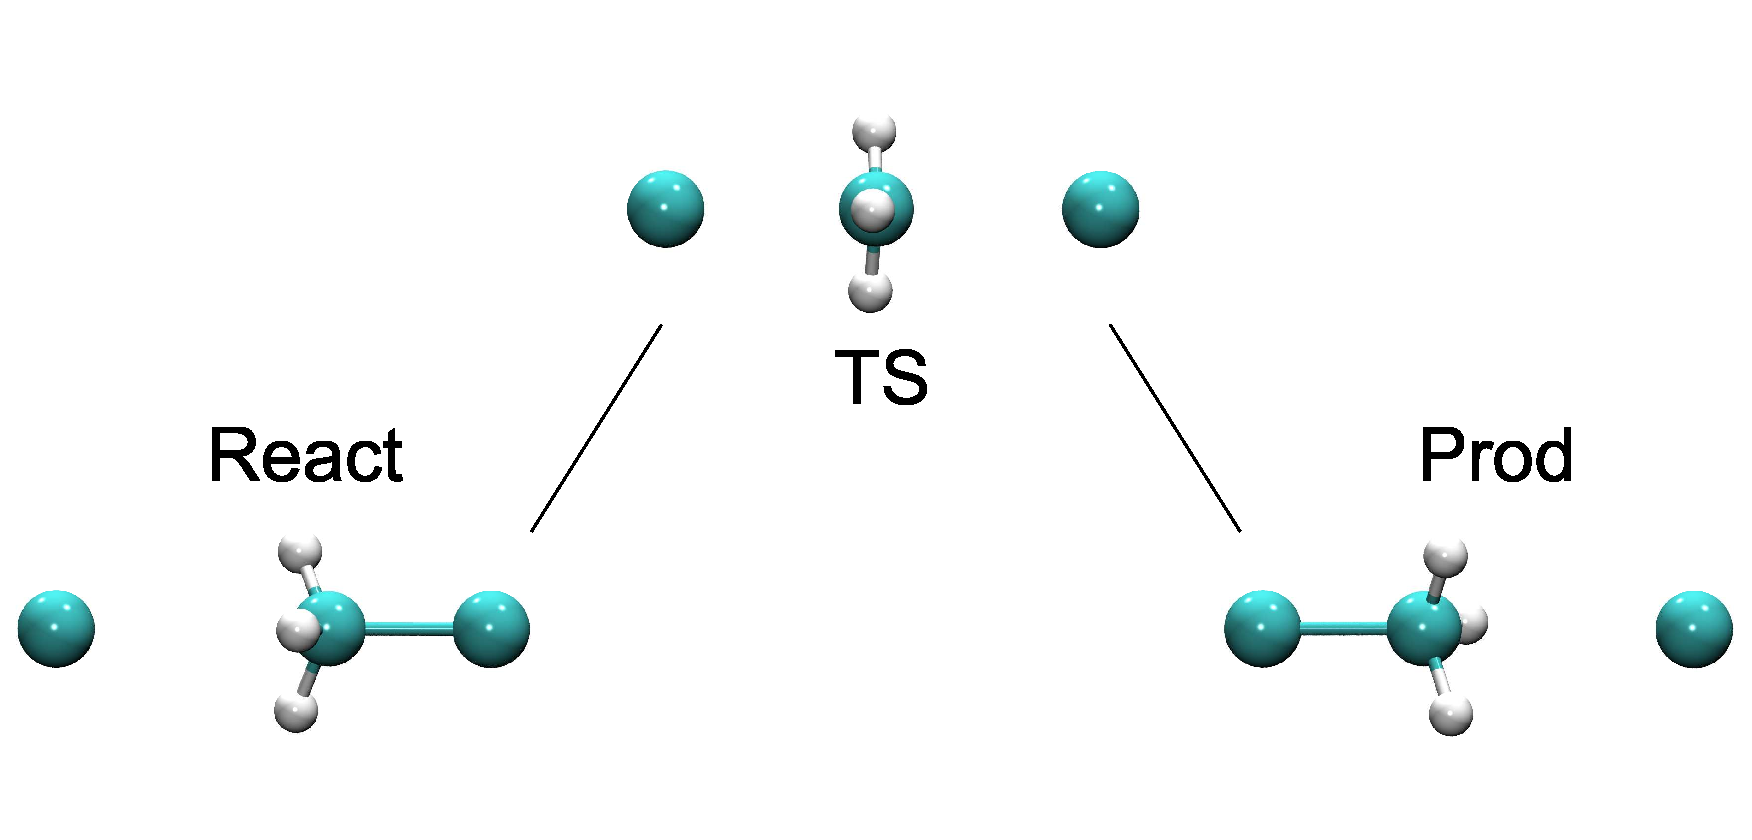
\includegraphics[width=\textwidth]{./pic/sn2_reaction.pdf}
\caption{A sketch of SN2 reaction}
\label{Fig_Reaction_sn2}
\end{center}
\end{figure*}

\subsection{Choice of CVs and simulation details}

The first thing you should decide is the collective variables (CVs) to be used:

\begin{itemize}
\item Distance?
\item Does the angle matter?
\item Torsion?
\item Coordination number?
\item Anything else?
\end{itemize}

Here we choose the bond length of C-Cl as CV1 and the bond length of C-Cl$^{-}$ as CV2. The simulation will be performed using the Born-Oppenheimer molecular dynamics (BO-MD) algorithm as implemented in the \qe\ program (\texttt{pw.x}) and then Car-Parrinello molecular dynamics (CP-MD) (\texttt{cp.x}). The electronic structure is computed within density functional theory (DFT) using the PBE exchange-correlation functional. Ultra-soft pseudo-potentials are used for the valence electrons, and the wave function is expanded in a plane waves basis set up to an kinetic energy cutoff of 25 Ry and charge density cutoff of 200 Ry. An orthorhombic P supercell of 18 * 12 * 12 a.u.$^{3}$ is used. The temperature of the system is 300 K via "soft" velocity rescaling in BO-MD and Nose-Hoover thermostat in CP-MD.

\subsection{Metadynamics with Born-Oppenheimer molecular dynamics}

For Metadynamics a possible input \texttt{plumed.dat} can be

\begin{verbatim}
# switching on metadynamics and Gaussian parameters
HILLS HEIGHT 0.001 W_STRIDE 2
# instruction for CVs printout
PRINT W_STRIDE 1
# the distance between C-Cl' and C-Cl
DISTANCE LIST 1 3 SIGMA 0.3
DISTANCE LIST 2 3 SIGMA 0.3
# WALLS: prevent to depart the two mols
UWALL CV 1 LIMIT 7.0 KAPPA 100.0
LWALL CV 1 LIMIT 2.5 KAPPA 100.0
UWALL CV 2 LIMIT 7.0 KAPPA 100.0
LWALL CV 2 LIMIT 2.5 KAPPA 100.0
# end of the input
ENDMETA
\end{verbatim}

Here we describe briefly the syntax used in the \texttt{PLUMED} input file. For the detail introduction, please have a look at the \texttt{PLUMED} manual\cite{PLUMED:manual}.

The symbol \# allows the user to comment any line in the input file. The \texttt{HILLS} turns on the standard Metadynamics and the \texttt{HEIGHT 0.001} means the height of the Gaussians is 0.001 Rdy. Pay attention: in this code distances are in Bohr (1 Bohr = 0.529177249 \AA) and the energies in Rydberg (1 Rydberg  = 13.60569 eV). The frequency for add Gaussians is controlled by \texttt{W\_STRIDE} followed by a number that represents the number of steps between one MD step and the other which is 2 here. The line that starts with the keyword \texttt{PRINT W\_STRIDE} control the frequency for the main \texttt{PLUMED} output file which is called \texttt{COLVAR}. This file contains the data regarding the collective variable positions, the constraint positions, the energy of hills and energy of constraints and other useful informations that will be introduced time by time during the tutorial. All the informations are appended in the \texttt{COLVAR} file and overwritten if an old \texttt{COLVAR} file already exists. The \texttt{DISTANCE LIST 1 3} shows that our CV1 is the distance between atom 1 and atom 3, the \texttt{SIGMA 0.3} indicates the width of the Gaussians is 0.3 Bohr. In order to prevent to depart the two molecules, we add the wall potentials on CV1 and CV2, for both of them the upper limit wall and the lower limit wall. The \texttt{UWALL} and \texttt{LWALL} keywords define a wall for the value of the CV s which limits the region of the phase space accessible during the simulation. The restraining potential starts acting on the system when the value of the CV is greater (in the case of \texttt{UWALL}) or lower (in the case of \texttt{LWALL}) than a certain limit \texttt{LIMIT}. The functional form of this potential is the following:

\begin{equation}
V_{wall}(s) = KAPPA (\frac{s - LIMIT + OFF}{EPS})^{EXP}
\label{EQ_vwall}
\end{equation}

where \texttt{KAPPA} is an energy constant in internal unit of the code, \texttt{EPS} a rescaling factor and \texttt{EXP} the exponent determining the power law. By default: \texttt{EXP} = 4, \texttt{EPS} = 1.0, \texttt{OFF} = 0.

The termination of the input for \texttt{PLUMED} is marked with the keyword \texttt{ENDMETA}. Whatever it follows is ignored by \texttt{PLUMED}. You can introduce blank lines. They are not interpreted by \texttt{PLUMED}.

Here is the input file pw.in for pw.x:

\begin{verbatim}
 &control
    title = 'ch3cl',
    calculation='md'
    restart_mode='from_scratch',
    pseudo_dir = './',
    outdir = './tmp',
    dt=20,
    nstep=2000,
    prefix = 'md',
 /
 &system
    ibrav = 8,
    celldm(1) = 18.d0,
    celldm(2) = 0.666666d0,
    celldm(3) = 0.666666d0,
    nat  = 6,
    ntyp = 3,
    tot_charge = -1,
    ecutwfc = 25.0,
    ecutrho = 100.0,
    nr1b = 24, nr2b = 24, nr3b = 24,
    nosym = .true.
 /

 &electrons
    conv_thr =  1.0d-8
    mixing_beta = 0.7
 /
 &ions
    pot_extrapolation='second-order'
    wfc_extrapolation='second-order'
    ion_temperature='berendsen'
    tempw= 300.
    nraise=20
 /
ATOMIC_SPECIES
 Cl 35.4527d0 Cl.blyp-mt.UPF
 C 12.0107d0 C.blyp-mt.UPF
 H 1.00794d0 H.blyp-vbc.UPF

ATOMIC_POSITIONS bohr
Cl      12.880706242   6.000000000   5.994035868
Cl       3.581982751   6.000000000   5.989431927
C        9.410606817   6.000000000   6.004535337
H        8.743333410   4.313700292   5.030609604
H        8.743333410   7.686299708   5.030609604
H        8.746264064   6.000000000   7.952930073

K_POINTS gamma
\end{verbatim}

In this example, we perform a 2000 steps NVT MD to reconstruct the free energy profile for the SN2 reaction. To run the metadynamics simulation, simply type

\begin{verbatim}
pw.x -plumed < pw.in > pw.out
\end{verbatim}

After the execution of the program, you will get a brunch of interesting stuff. First of all, you will get a \texttt{PLUMED.OUT} file that contains some printout from \texttt{PLUMED} so you may check whether the input was correctly read:

\begin{verbatim}
::::::::::::::::: READING PLUMED INPUT :::::::::::::::::
|-HILLS:
|--HEIGHT 0.001000  WRITING STRIDE 2 DEPOSITION RATE 0.000025 

|-PRINTING ON COLVAR FILE EVERY 1 STEPS
|-INITIAL TIME OFFSET IS 0.000000 TIME UNITS

1-DISTANCE: (1st SET: 1 ATOMS), (2nd SET: 1 ATOMS);  PBC ON SIGMA 0.300000
|- DISCARDING DISTANCE COMPONENTS (XYZ): 000
|- 1st SET MEMBERS:  1 
|- 2nd SET MEMBERS:  3 


2-DISTANCE: (1st SET: 1 ATOMS), (2nd SET: 1 ATOMS);  PBC ON SIGMA 0.300000
|- DISCARDING DISTANCE COMPONENTS (XYZ): 000
|- 1st SET MEMBERS:  2 
|- 2nd SET MEMBERS:  3 

|-WALL ON COLVAR 1: UPPER LIMIT = 7.000000, KAPPA = 100.000000, EXPONENT = 4,
 REDUX = 1.000000, OFFSET = 0.000000 

|-WALL ON COLVAR 1: LOWER LIMIT = 2.500000, KAPPA = 100.000000, EXPONENT = 4,
 REDUX = 1.000000, OFFSET = 0.000000 

|-WALL ON COLVAR 2: UPPER LIMIT = 7.000000, KAPPA = 100.000000, EXPONENT = 4,
 REDUX = 1.000000, OFFSET = 0.000000 

|-WALL ON COLVAR 2: LOWER LIMIT = 2.500000, KAPPA = 100.000000, EXPONENT = 4,
 REDUX = 1.000000, OFFSET = 0.000000 

|-HILLS ACTIVE ON COLVAR 1
|-HILLS ACTIVE ON COLVAR 2
\end{verbatim}

This tells you that everything is going fine. The index of atoms are parsed correctly and the printout is correctly understood. Now what you get is a \texttt{COLVAR} file that consists in the time evolution of the CVs. Its format looks something like this:

\begin{verbatim}
#! FIELDS time cv1 cv2 vbias vwall vext
     0.000      3.470115309      5.828643634      0.000000000      0.000000000
                0.000000000      0.000000000      0.000000000
    20.000      3.476912892      5.822800771      0.000000000      0.000000000
                0.000000000      0.000000000      0.000000000
    40.000      3.483516729      5.817608411      0.001000000      0.000000000
                0.000000000      0.000000000      0.000000000
    60.000      3.490411466      5.812574439      0.000999600      0.000000000
                0.000000000      0.000000000      0.000000000
    80.000      3.498291622      5.807005696      0.001998170      0.000000000
                0.000000000      0.000000000      0.000000000
   100.000      3.507739014      5.800326723      0.001994356      0.000000000
                0.000000000      0.000000000      0.000000000
\end{verbatim}

In the first line there is a simple remainder to the elements that you have in each column. Namely time first (in a.u. by default in \qe), then the value of the two CVs followed by the various additional potential energies introduced by \texttt{PLUMED}.  The fourth column is the bias potential, the wall potential is in the fifth column and the external potential is in the last. Now you can plot the evolution of the CVs with gnuplot by using the command \texttt{p "./COLVAR" u 1:2 t "CV1" ,"" u 1:3 t "CV2"} and you�ll get something like Fig. \ref{FIG_sn2_cv}. If you want to understand how the CVs are related then you may use the command \texttt{p "./COLVAR" u 2:3} with gnuplot that results in a plot like that in Fig. \ref{FIG_sn2_cvs}.

\begin{figure*}[htbp]
\begin{center}
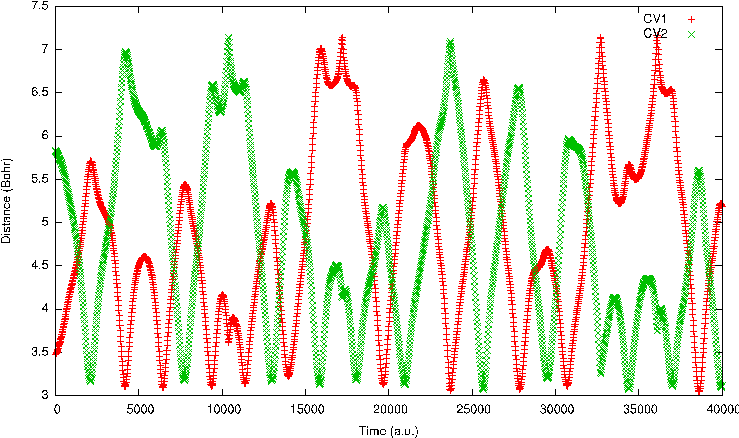
\includegraphics[width=\textwidth]{./pic/sn2cv.pdf}
\caption{The time evolution of CVs}
\label{FIG_sn2_cv}
\end{center}
\end{figure*}

\begin{figure*}[htbp]
\begin{center}
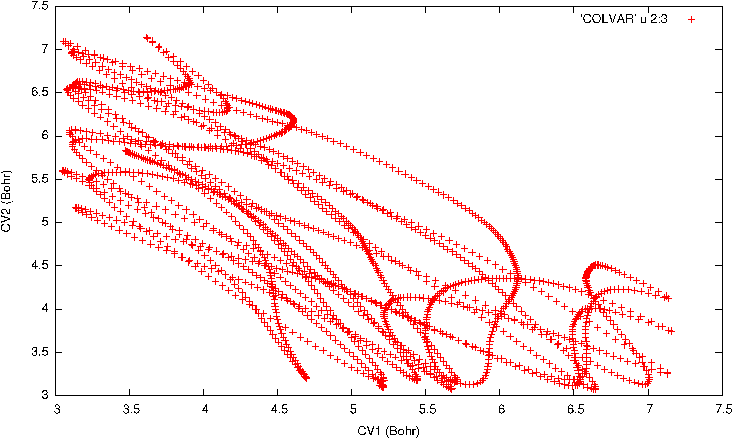
\includegraphics[width=\textwidth]{./pic/sn2cvs.pdf}
\caption{The time population of CVs}
\label{FIG_sn2_cvs}
\end{center}
\end{figure*}

Beside the usual \texttt{COLVAR} file, when you run a metadynamics calculation you get an additional file called \texttt{HILLS} which contains a list of the Gaussians deposited during the simulation. In the example above, this file looks like:

\begin{verbatim}
    40.000      3.483516729      5.817608411      0.300000000      0.300000000
                0.001000000   0.000 
    80.000      3.498291622      5.807005696      0.300000000      0.300000000
                0.001000000   0.000 
   120.000      3.519061248      5.792237732      0.300000000      0.300000000
                0.001000000   0.000 
   160.000      3.547107311      5.772092610      0.300000000      0.300000000
                0.001000000   0.000 
   200.000      3.578429291      5.750272190      0.300000000      0.300000000
                0.001000000   0.000 
   240.000      3.606928115      5.732241302      0.300000000      0.300000000
                0.001000000   0.000 
\end{verbatim}

where:

\begin{itemize}
\item the first column contains the time \texttt{t} (in internal unit of the MD code which is \texttt{a.u.} here in BOMD) at which the Gaussian was deposited;
\item the following 2 columns contain the centroid of the Gaussian, $S_{i}(R(t))$, one for each CV $i$;
\item the following 2 columns contain the Gaussian sigma $\sigma_{i}$, one for each CV $i$;
\item the last but one column contains the value of $W$;
\item the last column is meaningful only in well-tempered metadynamics simulations (see the next example).
\end{itemize}

This file will be used to calculate the estimate of the free energy at the end of our metadynamics calculation.

In order to restart a metadynamics run, the flag \texttt{RESTART} must be added to \texttt{plumed.dat} after flag \texttt{HILLS}. This allows a metadynamics simulation to be restarted after an interruption or after a run has finished. The \texttt{HILLS} files will be read at the beginning of the simulation and the bias potential applied to the dynamics. Note that the presence of the \texttt{RESTART} flag only affects the metadynamics part of the simulation, and thus the usual procedure for restarting a MD run must be followed.

\subsubsection{Free energy reconstruction}

In the long-time limit, the bias potential of metadynamics converges to the free energy changed in sign\cite{Bussi:2006gg}. At any time during the simulation we can sum the Gaussians deposited so far and obtain the current estimate of the free energy surface (FES) using the utility \texttt{sum\_hills} as we compiled in the previous section.

\begin{verbatim}
sum_hills.x -file HILLS -out fes.dat -ndim 2 -ngrid 100 100
\end{verbatim}

The file in output \texttt{fes.dat} contains the estimate of the free energy calculated on a regular grid whose dimension is specified by \texttt{-ngird}. These parameters should be chosen with care. To calculate accurately the potential in a given point of the CV space, a practical rule is to choose the bin size to be half the Gaussian sigma.

As usual, you can plot the 3D FES with gnuplot:

\begin{verbatim}
set pm3d
sp "fes.dat" w pm3d
\end{verbatim}

and you will get a plot like that in Fig. \ref{FIG_sn2_fes}

\begin{figure*}[htbp]
\begin{center}
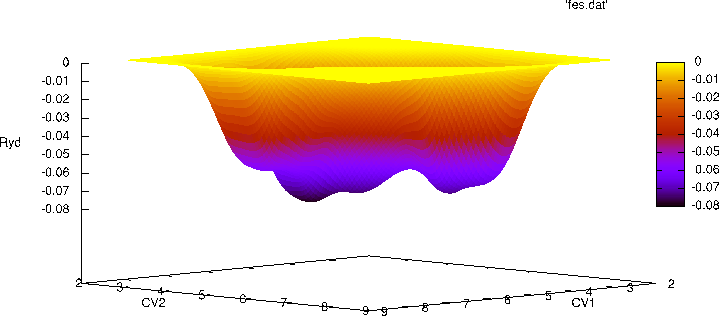
\includegraphics[width=\textwidth]{./pic/sn2_fes.pdf}
\caption{Free energy surface of SN2 reaction}
\label{FIG_sn2_fes}
\end{center}
\end{figure*}

\section{Second worked example: H-H}

In this example, well-tempered (WT) metadynamics\cite{Barducci:2008ua} will be employed to reconstruct the FES of the hydrogen molecule within Born-Oppenheimer approximation (with \texttt{pw.x}). In WT metadynamics, the Gaussian height $W$ is automatically rescaled during the simulations following:

\begin{equation}
W = W_{0} \exp{-\frac{V(S, t)}{k_{B}\Delta T}}
\label{EQ_wt}
\end{equation}

where $W_{0}$ is the initial Gaussian height and $\Delta T$ a parameter with the dimension of a temperature. The use of Eq. \ref{EQ_wt} guarantees that the bias potential converges in a single simulation and does not oscillate around the FES value, causing the problem of overfilling as what we got in Fig. \ref{FIG_sn2_fes}.

\begin{equation}
V(S, t\to \infty) = -\frac{\Delta T}{T + \Delta T} F(S) + C
\label{EQ_wt_v}
\end{equation}

where $T$ is the temperature of the system and $C$ a constant.

The quantity $T + \Delta T$ is often referred as the (fictitious) CV temperature, while the ratio $(T + \Delta T) / T$ as bias factor. For the details of WT metadynamics, please see references\cite{Barducci:2008ua, Laio:2008wu}. To perform a WT metadynamics simulation with \texttt{PLUMED} you have to use the directive \texttt{WELLTEMPERED} and specify one of the parameters described above using either the keyword \texttt{CV\_TEMPERTURE} or \texttt{BIASFACTOR}. In addition, the temperature of the system must be specified explicitly with \texttt{SIMTEMP}.

Here are some practical rules to choose wisely the parameters in WT metadynamics simulations:

\begin{itemize}
\item The bias factor (or equivalently the CV temperature) regulates how fast the amount of bias potential added decreases with simulation time and eventually controls the extent of exploration. The choice of these parameters depends on the typical free-energy barriers involved in the process under study. Note that this parameter can be changed on-the-fly as needed.
\item The optimal choice of the initial Gaussian height $W_{0}$ is less crucial and at the same time less trivial. It is irrelevant in the long time regime and affects only the transient part of the simulation. A short initial filling period can be desirable if the transverse degrees of freedom relax quickly, otherwise a moderate initial energy rate is a better choice.
\end{itemize}

The following is an example of input file for this WT metadynamics simulation at 300 K with a bias factor 10 and an initial Gaussian height of 0.005.

\begin{verbatim}
PRINT    W_STRIDE 5
HILLS    HEIGHT 0.005 W_STRIDE 10
WELLTEMPERED SIMTEMP 300 BIASFACTOR 10
DISTANCE LIST 1 2 SIGMA 0.2
ENDMETA
\end{verbatim}

In WT metadynamics, the Gaussians height as written in the \texttt{HILLS} file is multiplied by the factor $(T + \Delta T) / \Delta T$. This guarantees that when you sum the Gaussians (by means for example of the \texttt{sum\_hills} code) you get directly the FES. The last column of the \texttt{HILLS} file contains the value of the bias factor used in the WT metadynamics simulation. For this example, the \texttt{HILLS} file looks like:

\begin{verbatim}
   200.000      1.433853674      0.200000000      0.005555556   10.000 
   400.000      1.431075271      0.200000000      0.004147748   10.000 
   600.000      1.431419655      0.200000000      0.003334619   10.000 
   800.000      1.509148410      0.200000000      0.002937840   10.000 
  1000.000      1.683639369      0.200000000      0.003660780   10.000 
  1200.000      1.680674151      0.200000000      0.002997952   10.000 
\end{verbatim}

Then you can sum up the Gaussians and plot it with gnuplot.

\begin{verbatim}
sum_hills.x -ndim 1 -ndw 1 -file HILLS -out fes.dat
\end{verbatim}

The \texttt{sum\_hills} code could also be used to check the convergence of a metadynamics simulation. This can be easily achieved by calculating the estimate of the FES at regular interval in time using the \texttt{-stride} option and then evaluating the free energy at different time steps. Just run \texttt{sum\_hills}:

\begin{verbatim}
sum_hills.x -out fes.dat -ndim 1 -ndw 1 -stride 150
\end{verbatim}

and you will get \texttt{fes.dat}, the FES for the whole simulation and \texttt{fes.dat.1}, \texttt{fes.dat.2} ..., one every \texttt{stride} Gaussians. You can plot free energy estimate at different time steps as shown in Fig. \ref{FIG_hh_fes}.

\begin{figure*}[htbp]
\begin{center}
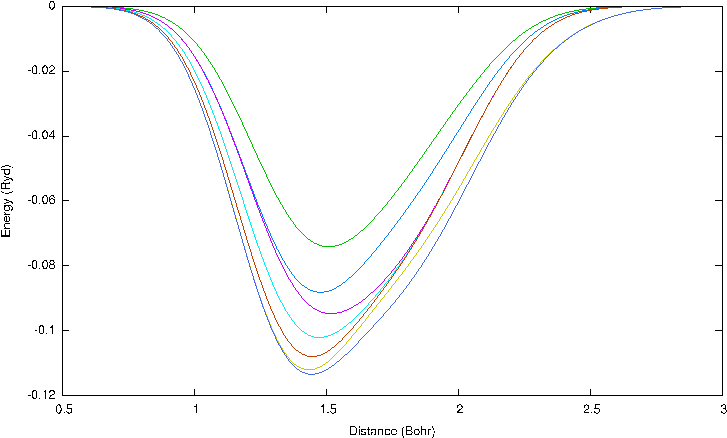
\includegraphics[width=\textwidth]{./pic/hh_fes.pdf}
\caption{Free energy surface}
\label{FIG_hh_fes}
\end{center}
\end{figure*}

From the Fig. \ref{FIG_hh_fes}, we can see that the lowest saddle point is at 1.43 Bohr, which is the bond length of the hydrogen molecule and it takes 0.113 Hartree = 3.09 eV to break this bond.

\newpage

\begin{thebibliography}{10}

\bibitem{Bonomi:2009ul} M. Bonomi, D. Branduardi, G. Bussi, C. Camilloni, D. Provasi, P. Raiteri, D. Donadio, F. Marinelli, F. Pietrucci, R.A. Broglia and M. Parrinello,  Comp. Phys. Comm. {\bf 180}, 1961 (2009).

\bibitem{Laio:2008wu} A. Laio and F. L. Gervasio, Rep. Prog. Phys., {\bf 71}, 126601 (2008).

\bibitem{Laio:2002wm} A. Laio and M. Parrinello, PNAS, {\bf 99}, 12562 (2002).

\bibitem{QE:guide} User's Guide for \qe: \texttt{espresso/Doc/}; \href{http://www.quantum-espresso.org/wp-content/uploads/Doc/user\_guide/}{http://www.quantum-espresso.org/wp-content/uploads/Doc/user\_guide}

\bibitem{PLUMED:manual} \texttt{PLUMED} manual: \href{https://sites.google.com/site/plumedweb/documentation}{https://sites.google.com/site/plumedweb/documentation}

\bibitem{Ensing:2005p53} B. Ensing, A. Laio, M. Parrinello, and M. L. Klein, J. Phys. Chem. B {\bf 109}, 6676 (2005).

\bibitem{Bussi:2006gg} G. Bussi, A. Laio and M. Parrinello, PRL {\bf 96}, 090601 (2006).

\bibitem{Barducci:2008ua} A. Barducci, G. Bussi and M. Parrinello, PRL {\bf 100},20603 (2008)

\end{thebibliography}

\end{document}
